\section{Notation}
%Placeholder parameters
%Prot. variants abbreviations (IDA, IWA, FGA, UC) (G2C3 and G2C4 as before)
%Term "source flit"

\section{Environment}
% 50,000 cycles (why?)
% Warmup and cooldown times (both 500 cycles)
% Injection rate of 0.2 into the network
In the experiments, a base network injection rate of 0.2 is assumed. This is the same value that \citeauthor{moriam18activeattackers} have chosen
\cite[2]{moriam18activeattackers} in order for the results to be comparable with their analyses. The actual injection rate may be higher as the base rate does not include the
issuance of \glspl{arq} and the resulting retransmissions.
\begin{itemize}
    \item Injection rate
        \begin{itemize}
            \item Value if 0.2 is realistic
            \item Possibility to generate pairs for fair comparison of UC/NC
            \item Base network injection rate of 0.2 is used for all experiments. The source flit creation rate is adjusted accordingly for the
                protocol variants to ensure that they have the same injection rate.
        \end{itemize}
    \item Overhead von Verschlüsselung+Auth vs. nur Auth vs keins von beiden (sowohl Latenz als auch Chipfläche)
\end{itemize}

\begin{table}
    \centering
    \begin{tabulary}{\textwidth}{C|C}
        Parameter name & Value \\\hline
        \Gls{noc} dimensions & 8x8 \\
        Clock frequency & 500 MHz \\
        Network base injection rate & 0.2 \\
        Simulation runtime & \num{50000} cycles \\
    \end{tabulary}
    \caption[short]{long}
    \label{tab:fixedparams}
\end{table}

\begin{table}
    \centering
    \begin{tabulary}{\textwidth}{C|C|C}
        Parameter name & Value range & Placeholder \\\hline
        Network coding & $\{\mathit{UC}, \mathit{G2C3}, \mathit{G2C4}\}$ & \pNCMode{} \\
        No. of encryption modules & $\mathbb{N}^*$ & \pEncMods{} \\
        No. of authentication modules & $\mathbb{N}^*$ & \pAuthMods{} \\
        \Gls{arq} limit & $[1, 2]$ & \pARQLimit{} \\
        \Gls{arq} timeout & $\mathbb{N}^*$ cycles & \pARQTimeout{} \\
        Routing strategy & $\{\mathit{\gls{dor}}, \mathit{\gls{dm}}, \mathit{\gls{romm}}, \mathit{\gls{ramm}}\}$ & \pRStrat{} \\
    \end{tabulary}
    \caption[short]{long}
    \label{tab:inputparams}
\end{table}

\section{Attacker Model}
\begin{itemize}
    \item Focuses on malicious modifications rather than DoS attacks
    \item Assumption: compromised routers → rely on NIs for security
    \item No protection against bandwidth depletion, but this is not the goal here
    \item Variable number of compromised routers (e.g. 8 for an 8x8 grid)
    \item Compromised routers randomly drop or modify packets (no intelligent modifications/drops)
    \item Reasoning for having only some compromised routers (in regard to the 3rd party NoC problem → why would they not make all routers the same?)
        → HT implies more logic in routers → more area and draws more power → might attract attention if all routers have this and overall NoC
        parameters diverge considerably from the expectations
\end{itemize}

Compromised routers: 6, 8, 23, 36, 46, 52, 59, 61 (8 routers randomly selected from the set of nodes with uniform probability distribution)

\section{Determining The Hyperparameters}
\subsection{ARQ Timeouts}\label{subsec:arqtimeouts}
In Section \ref{subsec:arqretransmissions}, the concept of \glspl{arq} and timeouts was introduced: receivers issue \glspl{arq} when the temporal gap
between the arrival of flits belonging to the same transmission unit becomes too large, i.e. when a timeout occurs. Its value is determined through
experiments and measured in clock cycles.

\begin{figure}
    \centering
    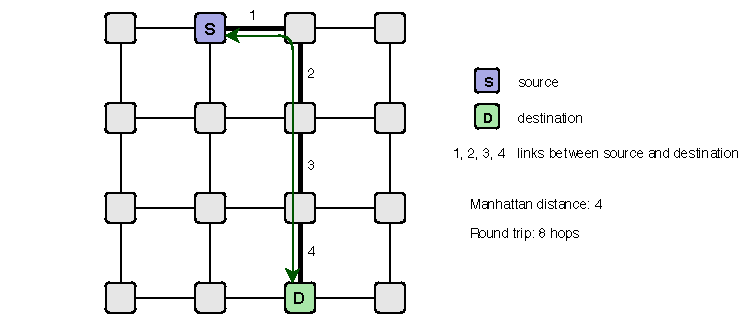
\includegraphics[width=0.9\textwidth]{arq-timeouts-calc}
    \caption[Example of ARQ timeout calculation]{Example for the calculation of \gls{arq} timeouts. With a Manhattan distance of 4 between source $S$ and
    destination $D$ and a given inter-arrival timeout $t_1$, the \gls{arq} timeout $t_2(S, D)$ is computed as $t_1 + 2 \cdot 4 = t_1 + 8$ cycles.}
    \label{fig:arqtimeoutscalc}
\end{figure}

In addition to the inter-arrival timeout, there is another, higher value that is used after an \gls{arq} was issued to await the answer, as explained
in Section \ref{subsec:arqretransmissions}. The \gls{arq} answer timeout depends on the inter-arrival timeout and the Manhattan distance between the
two affected communication partners. More precisely, if $t_1$ is the inter-arrival timeout, $t_2(S, D)$ is the \gls{arq} answer timeout for a
particular source $S$ and destination $D$, and $d$ is the Manhattan distance between the two nodes, then $t_2(S, D) = t_1 + 2 \cdot d$. Figure
\vref{fig:arqtimeoutscalc} illustrates this calculation.

Hence, only $t_1$ needs to be determined through experiments. Since this is the first parameter to be fixed, the other input values for the simulation
are estimated. The tests are independent of the protocol variant as the same injection rate is used for all of them. Table \vref{tab:setuparqtimeouts}
presents how the simulator is set up.

\begin{table}
    \centering
    \begin{tabulary}{\textwidth}{C|C|C|C|C|C|C|C|C}
        \pProtVar{} & \pNCMode{} & \pEncMods{} & \pAuthMods{} & \pARQLimit{} & \pARQTimeout{} & \pRStrat{} & \pNumAttackers{} & \pAttackProb{} \\\hline
        \gls{ida} & varying & 5 & 15 & 1 & varying & \gls{dor} & 0 & 0 \\
    \end{tabulary}
    \caption[Input parameters for ARQ timeouts experiment]{long}
    \label{tab:setuparqtimeouts}
\end{table}
% Why Ind. Auth.? Most flits per transmission unit (8 with G2C4)
% Why this number of enc./auth. units? Large number so there are definitely no internal congestions → area doesn't matter for this experiment
% Why ARQs per source flit and not per transmission unit? because size of trans. units varies considerably with prot. variant

To determine the timeout value, an uncompromised \gls{noc} (i.e., with zero malicious routers) is used. Ideally, no \glspl{arq} are issued in this
scenario. However, due to random deviations from the average flit injection rate, the network load varies over time and congestions in some routers
may occur. The resulting increased transmission delays may be high enough to trigger timeouts even when an \gls{arq} is not necessary. Sporadic
occurances of such cases cannot be ruled out, but should rarely happen. However, simply increasing the timeout until these cases vanish is undesirable
for two reasons. First, a high timeout directly corresponds to high latencies when flit losses necessitate \glspl{arq}. Second, the later an \gls{arq}
is issued, the larger the \gls{rtb} of the communication partner needs to be so that the flits in question are not already overwritten when the
\gls{arq} arrives. The goal of this experiment is to find a reasonable middle ground: the smallest timeout that does not entail a significant number of
unnecessary \glspl{arq} will be used for the subsequent evaluations.

\begin{figure}
    \centering
    % GNUPLOT: LaTeX picture with Postscript
\begingroup
\newcommand{\ft}[0]{\footnotesize}
  \makeatletter
  \providecommand\color[2][]{%
    \GenericError{(gnuplot) \space\space\space\@spaces}{%
      Package color not loaded in conjunction with
      terminal option `colourtext'%
    }{See the gnuplot documentation for explanation.%
    }{Either use 'blacktext' in gnuplot or load the package
      color.sty in LaTeX.}%
    \renewcommand\color[2][]{}%
  }%
  \providecommand\includegraphics[2][]{%
    \GenericError{(gnuplot) \space\space\space\@spaces}{%
      Package graphicx or graphics not loaded%
    }{See the gnuplot documentation for explanation.%
    }{The gnuplot epslatex terminal needs graphicx.sty or graphics.sty.}%
    \renewcommand\includegraphics[2][]{}%
  }%
  \providecommand\rotatebox[2]{#2}%
  \@ifundefined{ifGPcolor}{%
    \newif\ifGPcolor
    \GPcolortrue
  }{}%
  \@ifundefined{ifGPblacktext}{%
    \newif\ifGPblacktext
    \GPblacktextfalse
  }{}%
  % define a \g@addto@macro without @ in the name:
  \let\gplgaddtomacro\g@addto@macro
  % define empty templates for all commands taking text:
  \gdef\gplbacktext{}%
  \gdef\gplfronttext{}%
  \makeatother
  \ifGPblacktext
    % no textcolor at all
    \def\colorrgb#1{}%
    \def\colorgray#1{}%
  \else
    % gray or color?
    \ifGPcolor
      \def\colorrgb#1{\color[rgb]{#1}}%
      \def\colorgray#1{\color[gray]{#1}}%
      \expandafter\def\csname LTw\endcsname{\color{white}}%
      \expandafter\def\csname LTb\endcsname{\color{black}}%
      \expandafter\def\csname LTa\endcsname{\color{black}}%
      \expandafter\def\csname LT0\endcsname{\color[rgb]{1,0,0}}%
      \expandafter\def\csname LT1\endcsname{\color[rgb]{0,1,0}}%
      \expandafter\def\csname LT2\endcsname{\color[rgb]{0,0,1}}%
      \expandafter\def\csname LT3\endcsname{\color[rgb]{1,0,1}}%
      \expandafter\def\csname LT4\endcsname{\color[rgb]{0,1,1}}%
      \expandafter\def\csname LT5\endcsname{\color[rgb]{1,1,0}}%
      \expandafter\def\csname LT6\endcsname{\color[rgb]{0,0,0}}%
      \expandafter\def\csname LT7\endcsname{\color[rgb]{1,0.3,0}}%
      \expandafter\def\csname LT8\endcsname{\color[rgb]{0.5,0.5,0.5}}%
    \else
      % gray
      \def\colorrgb#1{\color{black}}%
      \def\colorgray#1{\color[gray]{#1}}%
      \expandafter\def\csname LTw\endcsname{\color{white}}%
      \expandafter\def\csname LTb\endcsname{\color{black}}%
      \expandafter\def\csname LTa\endcsname{\color{black}}%
      \expandafter\def\csname LT0\endcsname{\color{black}}%
      \expandafter\def\csname LT1\endcsname{\color{black}}%
      \expandafter\def\csname LT2\endcsname{\color{black}}%
      \expandafter\def\csname LT3\endcsname{\color{black}}%
      \expandafter\def\csname LT4\endcsname{\color{black}}%
      \expandafter\def\csname LT5\endcsname{\color{black}}%
      \expandafter\def\csname LT6\endcsname{\color{black}}%
      \expandafter\def\csname LT7\endcsname{\color{black}}%
      \expandafter\def\csname LT8\endcsname{\color{black}}%
    \fi
  \fi
    \setlength{\unitlength}{0.0500bp}%
    \ifx\gptboxheight\undefined%
      \newlength{\gptboxheight}%
      \newlength{\gptboxwidth}%
      \newsavebox{\gptboxtext}%
    \fi%
    \setlength{\fboxrule}{0.5pt}%
    \setlength{\fboxsep}{1pt}%
\begin{picture}(7920.00,3600.00)%
    \gplgaddtomacro\gplbacktext{%
      \csname LTb\endcsname%
      \put(946,704){\makebox(0,0)[r]{\strut{}$0$}}%
      \put(946,1230){\makebox(0,0)[r]{\strut{}$0.05$}}%
      \put(946,1756){\makebox(0,0)[r]{\strut{}$0.1$}}%
      \put(946,2283){\makebox(0,0)[r]{\strut{}$0.15$}}%
      \put(946,2809){\makebox(0,0)[r]{\strut{}$0.2$}}%
      \put(946,3335){\makebox(0,0)[r]{\strut{}$0.25$}}%
      \put(1615,484){\makebox(0,0){\strut{}$4$}}%
      \put(2689,484){\makebox(0,0){\strut{}$6$}}%
      \put(3763,484){\makebox(0,0){\strut{}$8$}}%
      \put(4838,484){\makebox(0,0){\strut{}$10$}}%
      \put(5912,484){\makebox(0,0){\strut{}$12$}}%
      \put(6986,484){\makebox(0,0){\strut{}$14$}}%
    }%
    \gplgaddtomacro\gplfronttext{%
      \csname LTb\endcsname%
      \put(176,2019){\rotatebox{-270}{\makebox(0,0){\strut{}\ft ARQs per source flit}}}%
      \put(4300,154){\makebox(0,0){\strut{}\ft Timeout in cycles}}%
      \csname LTb\endcsname%
      \put(6788,3197){\makebox(0,0)[r]{\strut{}\ft UC}}%
      \csname LTb\endcsname%
      \put(6788,3047){\makebox(0,0)[r]{\strut{}\ft G2C3}}%
      \csname LTb\endcsname%
      \put(6788,2897){\makebox(0,0)[r]{\strut{}\ft G2C4}}%
    }%
    \gplbacktext
    \put(0,0){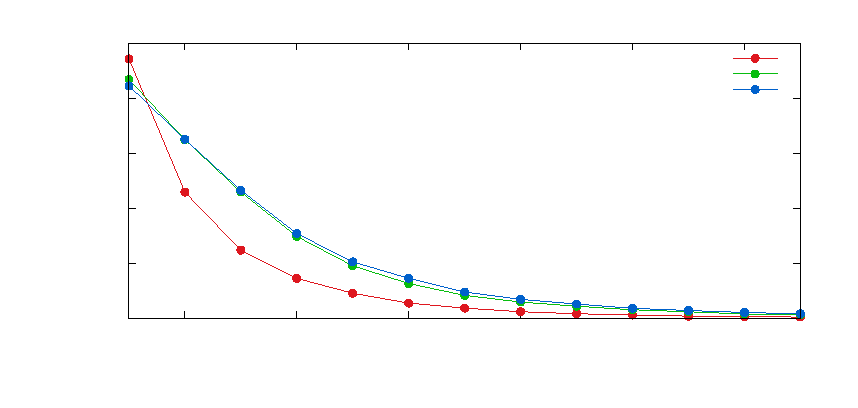
\includegraphics{../plots/arqtimeouts}}%
    \gplfronttext
  \end{picture}%
\endgroup

    \caption[Results for ARQ timeouts experiment]{long}
    \label{fig:resultsarqtimeouts}
\end{figure}

Figure \vref{fig:resultsarqtimeouts} shows the results for timeout values ranging from 3 to 15 cycles.

- Use sadias formula for RTB size estimation

We choose value of 12 because then for all NC variants, it is less than 1 ARQ per 100 source flits. Higher timeout would entail even less ARQs, but
increase latency and RTB sizes.

\subsection{Number Of Crypto Modules}
\begin{table}
    \centering
    \begin{tabulary}{\textwidth}{C|C|C|C|C|C|C|C|C}
        \pProtVar{} & \pNCMode{} & \pEncMods{} & \pAuthMods{} & \pARQLimit{} & \pARQTimeout{} & \pRStrat{} & \pNumAttackers{} & \pAttackProb{} \\\hline
        varying & varying & varying & varying & 1 & 12 & \gls{dor} & 8 & 0.2 \\
    \end{tabulary}
    \caption[Input parameters for number of crypto modules experiment]{long}
    \label{tab:setupnumcrypto}
\end{table}
- congestions in the queues in front of the crypto modules should be minimal
- less modules are better if possible because less chip area
- relatively high attack probabilities because more ARQs means more ver.+dec. retries at receivers, and network should be able to deal with that scenario
  "network needs to be equipped to deal with/handle periods of high traffic volumes"
- max. required enc. units: 4, because max. 2 flits can be drawn from the queues per cycle, so max. 4 flits active at the same time
- max. required auth. units: 12 (ind. auth), 10 (int. auth), 11 (gen. auth (2 flits = 11 cycles busy))
- criterion: max wait time needs to be 5 or less cycles

\begin{figure}
    \centering
    \begin{tabular}{ll}
        % GNUPLOT: LaTeX picture with Postscript
\begingroup
\newcommand{\ft}[0]{\footnotesize}\newcommand{\ty}[0]{\tiny}
  \makeatletter
  \providecommand\color[2][]{%
    \GenericError{(gnuplot) \space\space\space\@spaces}{%
      Package color not loaded in conjunction with
      terminal option `colourtext'%
    }{See the gnuplot documentation for explanation.%
    }{Either use 'blacktext' in gnuplot or load the package
      color.sty in LaTeX.}%
    \renewcommand\color[2][]{}%
  }%
  \providecommand\includegraphics[2][]{%
    \GenericError{(gnuplot) \space\space\space\@spaces}{%
      Package graphicx or graphics not loaded%
    }{See the gnuplot documentation for explanation.%
    }{The gnuplot epslatex terminal needs graphicx.sty or graphics.sty.}%
    \renewcommand\includegraphics[2][]{}%
  }%
  \providecommand\rotatebox[2]{#2}%
  \@ifundefined{ifGPcolor}{%
    \newif\ifGPcolor
    \GPcolortrue
  }{}%
  \@ifundefined{ifGPblacktext}{%
    \newif\ifGPblacktext
    \GPblacktextfalse
  }{}%
  % define a \g@addto@macro without @ in the name:
  \let\gplgaddtomacro\g@addto@macro
  % define empty templates for all commands taking text:
  \gdef\gplbacktext{}%
  \gdef\gplfronttext{}%
  \makeatother
  \ifGPblacktext
    % no textcolor at all
    \def\colorrgb#1{}%
    \def\colorgray#1{}%
  \else
    % gray or color?
    \ifGPcolor
      \def\colorrgb#1{\color[rgb]{#1}}%
      \def\colorgray#1{\color[gray]{#1}}%
      \expandafter\def\csname LTw\endcsname{\color{white}}%
      \expandafter\def\csname LTb\endcsname{\color{black}}%
      \expandafter\def\csname LTa\endcsname{\color{black}}%
      \expandafter\def\csname LT0\endcsname{\color[rgb]{1,0,0}}%
      \expandafter\def\csname LT1\endcsname{\color[rgb]{0,1,0}}%
      \expandafter\def\csname LT2\endcsname{\color[rgb]{0,0,1}}%
      \expandafter\def\csname LT3\endcsname{\color[rgb]{1,0,1}}%
      \expandafter\def\csname LT4\endcsname{\color[rgb]{0,1,1}}%
      \expandafter\def\csname LT5\endcsname{\color[rgb]{1,1,0}}%
      \expandafter\def\csname LT6\endcsname{\color[rgb]{0,0,0}}%
      \expandafter\def\csname LT7\endcsname{\color[rgb]{1,0.3,0}}%
      \expandafter\def\csname LT8\endcsname{\color[rgb]{0.5,0.5,0.5}}%
    \else
      % gray
      \def\colorrgb#1{\color{black}}%
      \def\colorgray#1{\color[gray]{#1}}%
      \expandafter\def\csname LTw\endcsname{\color{white}}%
      \expandafter\def\csname LTb\endcsname{\color{black}}%
      \expandafter\def\csname LTa\endcsname{\color{black}}%
      \expandafter\def\csname LT0\endcsname{\color{black}}%
      \expandafter\def\csname LT1\endcsname{\color{black}}%
      \expandafter\def\csname LT2\endcsname{\color{black}}%
      \expandafter\def\csname LT3\endcsname{\color{black}}%
      \expandafter\def\csname LT4\endcsname{\color{black}}%
      \expandafter\def\csname LT5\endcsname{\color{black}}%
      \expandafter\def\csname LT6\endcsname{\color{black}}%
      \expandafter\def\csname LT7\endcsname{\color{black}}%
      \expandafter\def\csname LT8\endcsname{\color{black}}%
    \fi
  \fi
    \setlength{\unitlength}{0.0500bp}%
    \ifx\gptboxheight\undefined%
      \newlength{\gptboxheight}%
      \newlength{\gptboxwidth}%
      \newsavebox{\gptboxtext}%
    \fi%
    \setlength{\fboxrule}{0.5pt}%
    \setlength{\fboxsep}{1pt}%
\begin{picture}(3600.00,3168.00)%
    \gplgaddtomacro\gplbacktext{%
      \csname LTb\endcsname%
      \put(858,660){\makebox(0,0)[r]{\strut{}\ft 1}}%
      \put(858,1782){\makebox(0,0)[r]{\strut{}\ft 10}}%
      \put(858,2903){\makebox(0,0)[r]{\strut{}\ft 100}}%
      \put(990,440){\makebox(0,0){\strut{}\ft 1}}%
      \put(1728,440){\makebox(0,0){\strut{}\ft 2}}%
      \put(2465,440){\makebox(0,0){\strut{}\ft 3}}%
      \put(3203,440){\makebox(0,0){\strut{}\ft 4}}%
    }%
    \gplgaddtomacro\gplfronttext{%
      \csname LTb\endcsname%
      \put(352,1781){\rotatebox{-270}{\makebox(0,0){\strut{}\ft Enqueued time in cycles}}}%
      \put(2096,154){\makebox(0,0){\strut{}\ft No. of encryption modules}}%
      \csname LTb\endcsname%
      \put(2468,2765){\makebox(0,0)[r]{\strut{}\ty IDA-UC max}}%
      \csname LTb\endcsname%
      \put(2468,2615){\makebox(0,0)[r]{\strut{}\ty avg}}%
      \csname LTb\endcsname%
      \put(2468,2465){\makebox(0,0)[r]{\strut{}\ty G2C3 max}}%
      \csname LTb\endcsname%
      \put(2468,2315){\makebox(0,0)[r]{\strut{}\ty avg}}%
      \csname LTb\endcsname%
      \put(2468,2165){\makebox(0,0)[r]{\strut{}\ty G2C4 max}}%
      \csname LTb\endcsname%
      \put(2468,2015){\makebox(0,0)[r]{\strut{}\ty avg}}%
    }%
    \gplbacktext
    \put(0,0){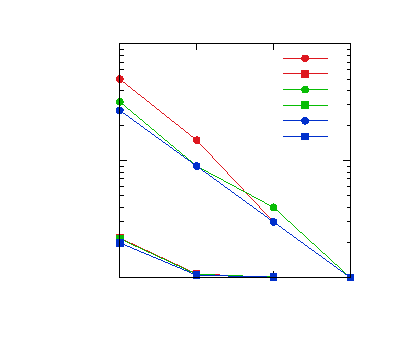
\includegraphics{../plots/encmodules-ida}}%
    \gplfronttext
  \end{picture}%
\endgroup
 & % GNUPLOT: LaTeX picture with Postscript
\begingroup
\newcommand{\ft}[0]{\footnotesize}\newcommand{\ty}[0]{\tiny}
  \makeatletter
  \providecommand\color[2][]{%
    \GenericError{(gnuplot) \space\space\space\@spaces}{%
      Package color not loaded in conjunction with
      terminal option `colourtext'%
    }{See the gnuplot documentation for explanation.%
    }{Either use 'blacktext' in gnuplot or load the package
      color.sty in LaTeX.}%
    \renewcommand\color[2][]{}%
  }%
  \providecommand\includegraphics[2][]{%
    \GenericError{(gnuplot) \space\space\space\@spaces}{%
      Package graphicx or graphics not loaded%
    }{See the gnuplot documentation for explanation.%
    }{The gnuplot epslatex terminal needs graphicx.sty or graphics.sty.}%
    \renewcommand\includegraphics[2][]{}%
  }%
  \providecommand\rotatebox[2]{#2}%
  \@ifundefined{ifGPcolor}{%
    \newif\ifGPcolor
    \GPcolortrue
  }{}%
  \@ifundefined{ifGPblacktext}{%
    \newif\ifGPblacktext
    \GPblacktextfalse
  }{}%
  % define a \g@addto@macro without @ in the name:
  \let\gplgaddtomacro\g@addto@macro
  % define empty templates for all commands taking text:
  \gdef\gplbacktext{}%
  \gdef\gplfronttext{}%
  \makeatother
  \ifGPblacktext
    % no textcolor at all
    \def\colorrgb#1{}%
    \def\colorgray#1{}%
  \else
    % gray or color?
    \ifGPcolor
      \def\colorrgb#1{\color[rgb]{#1}}%
      \def\colorgray#1{\color[gray]{#1}}%
      \expandafter\def\csname LTw\endcsname{\color{white}}%
      \expandafter\def\csname LTb\endcsname{\color{black}}%
      \expandafter\def\csname LTa\endcsname{\color{black}}%
      \expandafter\def\csname LT0\endcsname{\color[rgb]{1,0,0}}%
      \expandafter\def\csname LT1\endcsname{\color[rgb]{0,1,0}}%
      \expandafter\def\csname LT2\endcsname{\color[rgb]{0,0,1}}%
      \expandafter\def\csname LT3\endcsname{\color[rgb]{1,0,1}}%
      \expandafter\def\csname LT4\endcsname{\color[rgb]{0,1,1}}%
      \expandafter\def\csname LT5\endcsname{\color[rgb]{1,1,0}}%
      \expandafter\def\csname LT6\endcsname{\color[rgb]{0,0,0}}%
      \expandafter\def\csname LT7\endcsname{\color[rgb]{1,0.3,0}}%
      \expandafter\def\csname LT8\endcsname{\color[rgb]{0.5,0.5,0.5}}%
    \else
      % gray
      \def\colorrgb#1{\color{black}}%
      \def\colorgray#1{\color[gray]{#1}}%
      \expandafter\def\csname LTw\endcsname{\color{white}}%
      \expandafter\def\csname LTb\endcsname{\color{black}}%
      \expandafter\def\csname LTa\endcsname{\color{black}}%
      \expandafter\def\csname LT0\endcsname{\color{black}}%
      \expandafter\def\csname LT1\endcsname{\color{black}}%
      \expandafter\def\csname LT2\endcsname{\color{black}}%
      \expandafter\def\csname LT3\endcsname{\color{black}}%
      \expandafter\def\csname LT4\endcsname{\color{black}}%
      \expandafter\def\csname LT5\endcsname{\color{black}}%
      \expandafter\def\csname LT6\endcsname{\color{black}}%
      \expandafter\def\csname LT7\endcsname{\color{black}}%
      \expandafter\def\csname LT8\endcsname{\color{black}}%
    \fi
  \fi
    \setlength{\unitlength}{0.0500bp}%
    \ifx\gptboxheight\undefined%
      \newlength{\gptboxheight}%
      \newlength{\gptboxwidth}%
      \newsavebox{\gptboxtext}%
    \fi%
    \setlength{\fboxrule}{0.5pt}%
    \setlength{\fboxsep}{1pt}%
\begin{picture}(4464.00,3168.00)%
    \gplgaddtomacro\gplbacktext{%
      \csname LTb\endcsname%
      \put(858,660){\makebox(0,0)[r]{\strut{}\ft 1}}%
      \put(858,1782){\makebox(0,0)[r]{\strut{}\ft 10}}%
      \put(858,2903){\makebox(0,0)[r]{\strut{}\ft 100}}%
      \put(990,440){\makebox(0,0){\strut{}\ft 1}}%
      \put(1270,440){\makebox(0,0){\strut{}\ft 2}}%
      \put(1549,440){\makebox(0,0){\strut{}\ft 3}}%
      \put(1829,440){\makebox(0,0){\strut{}\ft 4}}%
      \put(2109,440){\makebox(0,0){\strut{}\ft 5}}%
      \put(2389,440){\makebox(0,0){\strut{}\ft 6}}%
      \put(2668,440){\makebox(0,0){\strut{}\ft 7}}%
      \put(2948,440){\makebox(0,0){\strut{}\ft 8}}%
      \put(3228,440){\makebox(0,0){\strut{}\ft 9}}%
      \put(3508,440){\makebox(0,0){\strut{}\ft 10}}%
      \put(3787,440){\makebox(0,0){\strut{}\ft 11}}%
      \put(4067,440){\makebox(0,0){\strut{}\ft 12}}%
    }%
    \gplgaddtomacro\gplfronttext{%
      \csname LTb\endcsname%
      \put(352,1781){\rotatebox{-270}{\makebox(0,0){\strut{}\ft Enqueued time in cycles}}}%
      \put(2528,154){\makebox(0,0){\strut{}\ft No. of authentication modules}}%
      \csname LTb\endcsname%
      \put(3332,2765){\makebox(0,0)[r]{\strut{}\ty IDA-UC max}}%
      \csname LTb\endcsname%
      \put(3332,2615){\makebox(0,0)[r]{\strut{}\ty avg}}%
      \csname LTb\endcsname%
      \put(3332,2465){\makebox(0,0)[r]{\strut{}\ty G2C3 max}}%
      \csname LTb\endcsname%
      \put(3332,2315){\makebox(0,0)[r]{\strut{}\ty avg}}%
      \csname LTb\endcsname%
      \put(3332,2165){\makebox(0,0)[r]{\strut{}\ty G2C4 max}}%
      \csname LTb\endcsname%
      \put(3332,2015){\makebox(0,0)[r]{\strut{}\ty avg}}%
    }%
    \gplbacktext
    \put(0,0){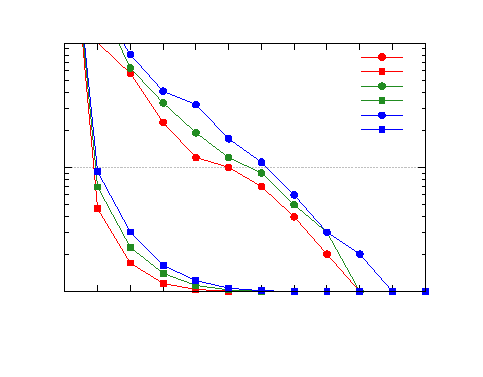
\includegraphics{../plots/authmodules-ida}}%
    \gplfronttext
  \end{picture}%
\endgroup
 \\
        % GNUPLOT: LaTeX picture with Postscript
\begingroup
\newcommand{\ft}[0]{\footnotesize}\newcommand{\ty}[0]{\tiny}
  \makeatletter
  \providecommand\color[2][]{%
    \GenericError{(gnuplot) \space\space\space\@spaces}{%
      Package color not loaded in conjunction with
      terminal option `colourtext'%
    }{See the gnuplot documentation for explanation.%
    }{Either use 'blacktext' in gnuplot or load the package
      color.sty in LaTeX.}%
    \renewcommand\color[2][]{}%
  }%
  \providecommand\includegraphics[2][]{%
    \GenericError{(gnuplot) \space\space\space\@spaces}{%
      Package graphicx or graphics not loaded%
    }{See the gnuplot documentation for explanation.%
    }{The gnuplot epslatex terminal needs graphicx.sty or graphics.sty.}%
    \renewcommand\includegraphics[2][]{}%
  }%
  \providecommand\rotatebox[2]{#2}%
  \@ifundefined{ifGPcolor}{%
    \newif\ifGPcolor
    \GPcolortrue
  }{}%
  \@ifundefined{ifGPblacktext}{%
    \newif\ifGPblacktext
    \GPblacktextfalse
  }{}%
  % define a \g@addto@macro without @ in the name:
  \let\gplgaddtomacro\g@addto@macro
  % define empty templates for all commands taking text:
  \gdef\gplbacktext{}%
  \gdef\gplfronttext{}%
  \makeatother
  \ifGPblacktext
    % no textcolor at all
    \def\colorrgb#1{}%
    \def\colorgray#1{}%
  \else
    % gray or color?
    \ifGPcolor
      \def\colorrgb#1{\color[rgb]{#1}}%
      \def\colorgray#1{\color[gray]{#1}}%
      \expandafter\def\csname LTw\endcsname{\color{white}}%
      \expandafter\def\csname LTb\endcsname{\color{black}}%
      \expandafter\def\csname LTa\endcsname{\color{black}}%
      \expandafter\def\csname LT0\endcsname{\color[rgb]{1,0,0}}%
      \expandafter\def\csname LT1\endcsname{\color[rgb]{0,1,0}}%
      \expandafter\def\csname LT2\endcsname{\color[rgb]{0,0,1}}%
      \expandafter\def\csname LT3\endcsname{\color[rgb]{1,0,1}}%
      \expandafter\def\csname LT4\endcsname{\color[rgb]{0,1,1}}%
      \expandafter\def\csname LT5\endcsname{\color[rgb]{1,1,0}}%
      \expandafter\def\csname LT6\endcsname{\color[rgb]{0,0,0}}%
      \expandafter\def\csname LT7\endcsname{\color[rgb]{1,0.3,0}}%
      \expandafter\def\csname LT8\endcsname{\color[rgb]{0.5,0.5,0.5}}%
    \else
      % gray
      \def\colorrgb#1{\color{black}}%
      \def\colorgray#1{\color[gray]{#1}}%
      \expandafter\def\csname LTw\endcsname{\color{white}}%
      \expandafter\def\csname LTb\endcsname{\color{black}}%
      \expandafter\def\csname LTa\endcsname{\color{black}}%
      \expandafter\def\csname LT0\endcsname{\color{black}}%
      \expandafter\def\csname LT1\endcsname{\color{black}}%
      \expandafter\def\csname LT2\endcsname{\color{black}}%
      \expandafter\def\csname LT3\endcsname{\color{black}}%
      \expandafter\def\csname LT4\endcsname{\color{black}}%
      \expandafter\def\csname LT5\endcsname{\color{black}}%
      \expandafter\def\csname LT6\endcsname{\color{black}}%
      \expandafter\def\csname LT7\endcsname{\color{black}}%
      \expandafter\def\csname LT8\endcsname{\color{black}}%
    \fi
  \fi
    \setlength{\unitlength}{0.0500bp}%
    \ifx\gptboxheight\undefined%
      \newlength{\gptboxheight}%
      \newlength{\gptboxwidth}%
      \newsavebox{\gptboxtext}%
    \fi%
    \setlength{\fboxrule}{0.5pt}%
    \setlength{\fboxsep}{1pt}%
\begin{picture}(3600.00,3168.00)%
    \gplgaddtomacro\gplbacktext{%
      \csname LTb\endcsname%
      \put(858,660){\makebox(0,0)[r]{\strut{}\ft 1}}%
      \put(858,1782){\makebox(0,0)[r]{\strut{}\ft 10}}%
      \put(858,2903){\makebox(0,0)[r]{\strut{}\ft 100}}%
      \put(990,440){\makebox(0,0){\strut{}\ft 1}}%
      \put(1728,440){\makebox(0,0){\strut{}\ft 2}}%
      \put(2465,440){\makebox(0,0){\strut{}\ft 3}}%
      \put(3203,440){\makebox(0,0){\strut{}\ft 4}}%
    }%
    \gplgaddtomacro\gplfronttext{%
      \csname LTb\endcsname%
      \put(352,1781){\rotatebox{-270}{\makebox(0,0){\strut{}\ft Enqueued time in cycles}}}%
      \put(2096,154){\makebox(0,0){\strut{}\ft No. of encryption modules}}%
      \csname LTb\endcsname%
      \put(2468,2765){\makebox(0,0)[r]{\strut{}\ty IWA-UC max}}%
      \csname LTb\endcsname%
      \put(2468,2615){\makebox(0,0)[r]{\strut{}\ty avg}}%
      \csname LTb\endcsname%
      \put(2468,2465){\makebox(0,0)[r]{\strut{}\ty G2C3 max}}%
      \csname LTb\endcsname%
      \put(2468,2315){\makebox(0,0)[r]{\strut{}\ty avg}}%
      \csname LTb\endcsname%
      \put(2468,2165){\makebox(0,0)[r]{\strut{}\ty G2C4 max}}%
      \csname LTb\endcsname%
      \put(2468,2015){\makebox(0,0)[r]{\strut{}\ty avg}}%
    }%
    \gplbacktext
    \put(0,0){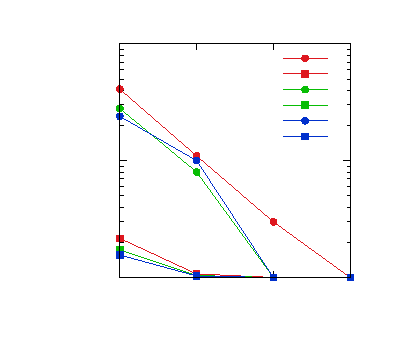
\includegraphics{../plots/encmodules-iwa}}%
    \gplfronttext
  \end{picture}%
\endgroup
 & % GNUPLOT: LaTeX picture with Postscript
\begingroup
\newcommand{\ft}[0]{\footnotesize}\newcommand{\ty}[0]{\tiny}
  \makeatletter
  \providecommand\color[2][]{%
    \GenericError{(gnuplot) \space\space\space\@spaces}{%
      Package color not loaded in conjunction with
      terminal option `colourtext'%
    }{See the gnuplot documentation for explanation.%
    }{Either use 'blacktext' in gnuplot or load the package
      color.sty in LaTeX.}%
    \renewcommand\color[2][]{}%
  }%
  \providecommand\includegraphics[2][]{%
    \GenericError{(gnuplot) \space\space\space\@spaces}{%
      Package graphicx or graphics not loaded%
    }{See the gnuplot documentation for explanation.%
    }{The gnuplot epslatex terminal needs graphicx.sty or graphics.sty.}%
    \renewcommand\includegraphics[2][]{}%
  }%
  \providecommand\rotatebox[2]{#2}%
  \@ifundefined{ifGPcolor}{%
    \newif\ifGPcolor
    \GPcolortrue
  }{}%
  \@ifundefined{ifGPblacktext}{%
    \newif\ifGPblacktext
    \GPblacktextfalse
  }{}%
  % define a \g@addto@macro without @ in the name:
  \let\gplgaddtomacro\g@addto@macro
  % define empty templates for all commands taking text:
  \gdef\gplbacktext{}%
  \gdef\gplfronttext{}%
  \makeatother
  \ifGPblacktext
    % no textcolor at all
    \def\colorrgb#1{}%
    \def\colorgray#1{}%
  \else
    % gray or color?
    \ifGPcolor
      \def\colorrgb#1{\color[rgb]{#1}}%
      \def\colorgray#1{\color[gray]{#1}}%
      \expandafter\def\csname LTw\endcsname{\color{white}}%
      \expandafter\def\csname LTb\endcsname{\color{black}}%
      \expandafter\def\csname LTa\endcsname{\color{black}}%
      \expandafter\def\csname LT0\endcsname{\color[rgb]{1,0,0}}%
      \expandafter\def\csname LT1\endcsname{\color[rgb]{0,1,0}}%
      \expandafter\def\csname LT2\endcsname{\color[rgb]{0,0,1}}%
      \expandafter\def\csname LT3\endcsname{\color[rgb]{1,0,1}}%
      \expandafter\def\csname LT4\endcsname{\color[rgb]{0,1,1}}%
      \expandafter\def\csname LT5\endcsname{\color[rgb]{1,1,0}}%
      \expandafter\def\csname LT6\endcsname{\color[rgb]{0,0,0}}%
      \expandafter\def\csname LT7\endcsname{\color[rgb]{1,0.3,0}}%
      \expandafter\def\csname LT8\endcsname{\color[rgb]{0.5,0.5,0.5}}%
    \else
      % gray
      \def\colorrgb#1{\color{black}}%
      \def\colorgray#1{\color[gray]{#1}}%
      \expandafter\def\csname LTw\endcsname{\color{white}}%
      \expandafter\def\csname LTb\endcsname{\color{black}}%
      \expandafter\def\csname LTa\endcsname{\color{black}}%
      \expandafter\def\csname LT0\endcsname{\color{black}}%
      \expandafter\def\csname LT1\endcsname{\color{black}}%
      \expandafter\def\csname LT2\endcsname{\color{black}}%
      \expandafter\def\csname LT3\endcsname{\color{black}}%
      \expandafter\def\csname LT4\endcsname{\color{black}}%
      \expandafter\def\csname LT5\endcsname{\color{black}}%
      \expandafter\def\csname LT6\endcsname{\color{black}}%
      \expandafter\def\csname LT7\endcsname{\color{black}}%
      \expandafter\def\csname LT8\endcsname{\color{black}}%
    \fi
  \fi
    \setlength{\unitlength}{0.0500bp}%
    \ifx\gptboxheight\undefined%
      \newlength{\gptboxheight}%
      \newlength{\gptboxwidth}%
      \newsavebox{\gptboxtext}%
    \fi%
    \setlength{\fboxrule}{0.5pt}%
    \setlength{\fboxsep}{1pt}%
\begin{picture}(4464.00,3168.00)%
    \gplgaddtomacro\gplbacktext{%
      \csname LTb\endcsname%
      \put(858,660){\makebox(0,0)[r]{\strut{}\ft 1}}%
      \put(858,1782){\makebox(0,0)[r]{\strut{}\ft 10}}%
      \put(858,2903){\makebox(0,0)[r]{\strut{}\ft 100}}%
      \put(990,440){\makebox(0,0){\strut{}\ft 1}}%
      \put(1270,440){\makebox(0,0){\strut{}\ft 2}}%
      \put(1549,440){\makebox(0,0){\strut{}\ft 3}}%
      \put(1829,440){\makebox(0,0){\strut{}\ft 4}}%
      \put(2109,440){\makebox(0,0){\strut{}\ft 5}}%
      \put(2389,440){\makebox(0,0){\strut{}\ft 6}}%
      \put(2668,440){\makebox(0,0){\strut{}\ft 7}}%
      \put(2948,440){\makebox(0,0){\strut{}\ft 8}}%
      \put(3228,440){\makebox(0,0){\strut{}\ft 9}}%
      \put(3508,440){\makebox(0,0){\strut{}\ft 10}}%
      \put(3787,440){\makebox(0,0){\strut{}\ft 11}}%
      \put(4067,440){\makebox(0,0){\strut{}\ft 12}}%
    }%
    \gplgaddtomacro\gplfronttext{%
      \csname LTb\endcsname%
      \put(352,1781){\rotatebox{-270}{\makebox(0,0){\strut{}\ft Enqueued time in cycles}}}%
      \put(2528,154){\makebox(0,0){\strut{}\ft No. of authentication modules}}%
      \csname LTb\endcsname%
      \put(3332,2765){\makebox(0,0)[r]{\strut{}\ty IWA-UC max}}%
      \csname LTb\endcsname%
      \put(3332,2615){\makebox(0,0)[r]{\strut{}\ty avg}}%
      \csname LTb\endcsname%
      \put(3332,2465){\makebox(0,0)[r]{\strut{}\ty G2C3 max}}%
      \csname LTb\endcsname%
      \put(3332,2315){\makebox(0,0)[r]{\strut{}\ty avg}}%
      \csname LTb\endcsname%
      \put(3332,2165){\makebox(0,0)[r]{\strut{}\ty G2C4 max}}%
      \csname LTb\endcsname%
      \put(3332,2015){\makebox(0,0)[r]{\strut{}\ty avg}}%
    }%
    \gplbacktext
    \put(0,0){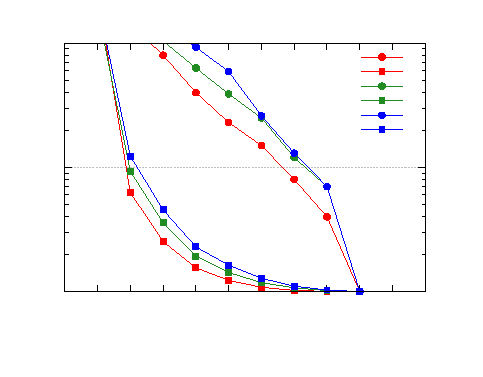
\includegraphics{../plots/authmodules-iwa}}%
    \gplfronttext
  \end{picture}%
\endgroup
 \\
        % GNUPLOT: LaTeX picture with Postscript
\begingroup
\newcommand{\ft}[0]{\footnotesize}\newcommand{\ty}[0]{\tiny}
  \makeatletter
  \providecommand\color[2][]{%
    \GenericError{(gnuplot) \space\space\space\@spaces}{%
      Package color not loaded in conjunction with
      terminal option `colourtext'%
    }{See the gnuplot documentation for explanation.%
    }{Either use 'blacktext' in gnuplot or load the package
      color.sty in LaTeX.}%
    \renewcommand\color[2][]{}%
  }%
  \providecommand\includegraphics[2][]{%
    \GenericError{(gnuplot) \space\space\space\@spaces}{%
      Package graphicx or graphics not loaded%
    }{See the gnuplot documentation for explanation.%
    }{The gnuplot epslatex terminal needs graphicx.sty or graphics.sty.}%
    \renewcommand\includegraphics[2][]{}%
  }%
  \providecommand\rotatebox[2]{#2}%
  \@ifundefined{ifGPcolor}{%
    \newif\ifGPcolor
    \GPcolortrue
  }{}%
  \@ifundefined{ifGPblacktext}{%
    \newif\ifGPblacktext
    \GPblacktextfalse
  }{}%
  % define a \g@addto@macro without @ in the name:
  \let\gplgaddtomacro\g@addto@macro
  % define empty templates for all commands taking text:
  \gdef\gplbacktext{}%
  \gdef\gplfronttext{}%
  \makeatother
  \ifGPblacktext
    % no textcolor at all
    \def\colorrgb#1{}%
    \def\colorgray#1{}%
  \else
    % gray or color?
    \ifGPcolor
      \def\colorrgb#1{\color[rgb]{#1}}%
      \def\colorgray#1{\color[gray]{#1}}%
      \expandafter\def\csname LTw\endcsname{\color{white}}%
      \expandafter\def\csname LTb\endcsname{\color{black}}%
      \expandafter\def\csname LTa\endcsname{\color{black}}%
      \expandafter\def\csname LT0\endcsname{\color[rgb]{1,0,0}}%
      \expandafter\def\csname LT1\endcsname{\color[rgb]{0,1,0}}%
      \expandafter\def\csname LT2\endcsname{\color[rgb]{0,0,1}}%
      \expandafter\def\csname LT3\endcsname{\color[rgb]{1,0,1}}%
      \expandafter\def\csname LT4\endcsname{\color[rgb]{0,1,1}}%
      \expandafter\def\csname LT5\endcsname{\color[rgb]{1,1,0}}%
      \expandafter\def\csname LT6\endcsname{\color[rgb]{0,0,0}}%
      \expandafter\def\csname LT7\endcsname{\color[rgb]{1,0.3,0}}%
      \expandafter\def\csname LT8\endcsname{\color[rgb]{0.5,0.5,0.5}}%
    \else
      % gray
      \def\colorrgb#1{\color{black}}%
      \def\colorgray#1{\color[gray]{#1}}%
      \expandafter\def\csname LTw\endcsname{\color{white}}%
      \expandafter\def\csname LTb\endcsname{\color{black}}%
      \expandafter\def\csname LTa\endcsname{\color{black}}%
      \expandafter\def\csname LT0\endcsname{\color{black}}%
      \expandafter\def\csname LT1\endcsname{\color{black}}%
      \expandafter\def\csname LT2\endcsname{\color{black}}%
      \expandafter\def\csname LT3\endcsname{\color{black}}%
      \expandafter\def\csname LT4\endcsname{\color{black}}%
      \expandafter\def\csname LT5\endcsname{\color{black}}%
      \expandafter\def\csname LT6\endcsname{\color{black}}%
      \expandafter\def\csname LT7\endcsname{\color{black}}%
      \expandafter\def\csname LT8\endcsname{\color{black}}%
    \fi
  \fi
    \setlength{\unitlength}{0.0500bp}%
    \ifx\gptboxheight\undefined%
      \newlength{\gptboxheight}%
      \newlength{\gptboxwidth}%
      \newsavebox{\gptboxtext}%
    \fi%
    \setlength{\fboxrule}{0.5pt}%
    \setlength{\fboxsep}{1pt}%
\begin{picture}(3600.00,3168.00)%
    \gplgaddtomacro\gplbacktext{%
      \csname LTb\endcsname%
      \put(858,660){\makebox(0,0)[r]{\strut{}\ft 1}}%
      \put(858,1782){\makebox(0,0)[r]{\strut{}\ft 10}}%
      \put(858,2903){\makebox(0,0)[r]{\strut{}\ft 100}}%
      \put(990,440){\makebox(0,0){\strut{}\ft 1}}%
      \put(1728,440){\makebox(0,0){\strut{}\ft 2}}%
      \put(2465,440){\makebox(0,0){\strut{}\ft 3}}%
      \put(3203,440){\makebox(0,0){\strut{}\ft 4}}%
    }%
    \gplgaddtomacro\gplfronttext{%
      \csname LTb\endcsname%
      \put(352,1781){\rotatebox{-270}{\makebox(0,0){\strut{}\ft Enqueued time in cycles}}}%
      \put(2096,154){\makebox(0,0){\strut{}\ft No. of encryption modules}}%
      \csname LTb\endcsname%
      \put(2468,2765){\makebox(0,0)[r]{\strut{}\ty FGA-G2C3 max}}%
      \csname LTb\endcsname%
      \put(2468,2615){\makebox(0,0)[r]{\strut{}\ty avg}}%
      \csname LTb\endcsname%
      \put(2468,2465){\makebox(0,0)[r]{\strut{}\ty G2C4 max}}%
      \csname LTb\endcsname%
      \put(2468,2315){\makebox(0,0)[r]{\strut{}\ty avg}}%
    }%
    \gplbacktext
    \put(0,0){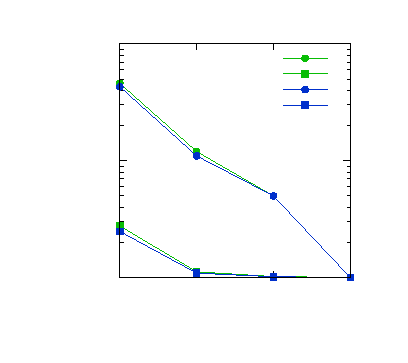
\includegraphics{../plots/encmodules-fga}}%
    \gplfronttext
  \end{picture}%
\endgroup
 & % GNUPLOT: LaTeX picture with Postscript
\begingroup
\newcommand{\ft}[0]{\footnotesize}\newcommand{\ty}[0]{\tiny}
  \makeatletter
  \providecommand\color[2][]{%
    \GenericError{(gnuplot) \space\space\space\@spaces}{%
      Package color not loaded in conjunction with
      terminal option `colourtext'%
    }{See the gnuplot documentation for explanation.%
    }{Either use 'blacktext' in gnuplot or load the package
      color.sty in LaTeX.}%
    \renewcommand\color[2][]{}%
  }%
  \providecommand\includegraphics[2][]{%
    \GenericError{(gnuplot) \space\space\space\@spaces}{%
      Package graphicx or graphics not loaded%
    }{See the gnuplot documentation for explanation.%
    }{The gnuplot epslatex terminal needs graphicx.sty or graphics.sty.}%
    \renewcommand\includegraphics[2][]{}%
  }%
  \providecommand\rotatebox[2]{#2}%
  \@ifundefined{ifGPcolor}{%
    \newif\ifGPcolor
    \GPcolortrue
  }{}%
  \@ifundefined{ifGPblacktext}{%
    \newif\ifGPblacktext
    \GPblacktextfalse
  }{}%
  % define a \g@addto@macro without @ in the name:
  \let\gplgaddtomacro\g@addto@macro
  % define empty templates for all commands taking text:
  \gdef\gplbacktext{}%
  \gdef\gplfronttext{}%
  \makeatother
  \ifGPblacktext
    % no textcolor at all
    \def\colorrgb#1{}%
    \def\colorgray#1{}%
  \else
    % gray or color?
    \ifGPcolor
      \def\colorrgb#1{\color[rgb]{#1}}%
      \def\colorgray#1{\color[gray]{#1}}%
      \expandafter\def\csname LTw\endcsname{\color{white}}%
      \expandafter\def\csname LTb\endcsname{\color{black}}%
      \expandafter\def\csname LTa\endcsname{\color{black}}%
      \expandafter\def\csname LT0\endcsname{\color[rgb]{1,0,0}}%
      \expandafter\def\csname LT1\endcsname{\color[rgb]{0,1,0}}%
      \expandafter\def\csname LT2\endcsname{\color[rgb]{0,0,1}}%
      \expandafter\def\csname LT3\endcsname{\color[rgb]{1,0,1}}%
      \expandafter\def\csname LT4\endcsname{\color[rgb]{0,1,1}}%
      \expandafter\def\csname LT5\endcsname{\color[rgb]{1,1,0}}%
      \expandafter\def\csname LT6\endcsname{\color[rgb]{0,0,0}}%
      \expandafter\def\csname LT7\endcsname{\color[rgb]{1,0.3,0}}%
      \expandafter\def\csname LT8\endcsname{\color[rgb]{0.5,0.5,0.5}}%
    \else
      % gray
      \def\colorrgb#1{\color{black}}%
      \def\colorgray#1{\color[gray]{#1}}%
      \expandafter\def\csname LTw\endcsname{\color{white}}%
      \expandafter\def\csname LTb\endcsname{\color{black}}%
      \expandafter\def\csname LTa\endcsname{\color{black}}%
      \expandafter\def\csname LT0\endcsname{\color{black}}%
      \expandafter\def\csname LT1\endcsname{\color{black}}%
      \expandafter\def\csname LT2\endcsname{\color{black}}%
      \expandafter\def\csname LT3\endcsname{\color{black}}%
      \expandafter\def\csname LT4\endcsname{\color{black}}%
      \expandafter\def\csname LT5\endcsname{\color{black}}%
      \expandafter\def\csname LT6\endcsname{\color{black}}%
      \expandafter\def\csname LT7\endcsname{\color{black}}%
      \expandafter\def\csname LT8\endcsname{\color{black}}%
    \fi
  \fi
    \setlength{\unitlength}{0.0500bp}%
    \ifx\gptboxheight\undefined%
      \newlength{\gptboxheight}%
      \newlength{\gptboxwidth}%
      \newsavebox{\gptboxtext}%
    \fi%
    \setlength{\fboxrule}{0.5pt}%
    \setlength{\fboxsep}{1pt}%
\begin{picture}(4320.00,3310.00)%
    \gplgaddtomacro\gplbacktext{%
      \csname LTb\endcsname%
      \put(330,660){\makebox(0,0)[r]{\strut{}\ft 1}}%
      \csname LTb\endcsname%
      \put(330,1853){\makebox(0,0)[r]{\strut{}\ft 10}}%
      \csname LTb\endcsname%
      \put(330,3045){\makebox(0,0)[r]{\strut{}\ft 100}}%
      \put(462,440){\makebox(0,0){\strut{}\ft 1}}%
      \put(777,440){\makebox(0,0){\strut{}\ft 2}}%
      \put(1091,440){\makebox(0,0){\strut{}\ft 3}}%
      \put(1406,440){\makebox(0,0){\strut{}\ft 4}}%
      \put(1721,440){\makebox(0,0){\strut{}\ft 5}}%
      \put(2035,440){\makebox(0,0){\strut{}\ft 6}}%
      \put(2350,440){\makebox(0,0){\strut{}\ft 7}}%
      \put(2664,440){\makebox(0,0){\strut{}\ft 8}}%
      \put(2979,440){\makebox(0,0){\strut{}\ft 9}}%
      \put(3294,440){\makebox(0,0){\strut{}\ft 10}}%
      \put(3608,440){\makebox(0,0){\strut{}\ft 11}}%
      \put(3923,440){\makebox(0,0){\strut{}\ft 12}}%
    }%
    \gplgaddtomacro\gplfronttext{%
      \csname LTb\endcsname%
      \put(-137,1852){\rotatebox{-270}{\makebox(0,0){\strut{}\ft Enqueued time in cycles}}}%
      \put(2192,154){\makebox(0,0){\strut{}\ft No. of authentication modules}}%
      \csname LTb\endcsname%
      \put(3224,2912){\makebox(0,0)[r]{\strut{}\ty FGA-G2C3 max}}%
      \csname LTb\endcsname%
      \put(3224,2772){\makebox(0,0)[r]{\strut{}\ty avg}}%
      \csname LTb\endcsname%
      \put(3224,2632){\makebox(0,0)[r]{\strut{}\ty G2C4 max}}%
      \csname LTb\endcsname%
      \put(3224,2492){\makebox(0,0)[r]{\strut{}\ty avg}}%
    }%
    \gplbacktext
    \put(0,0){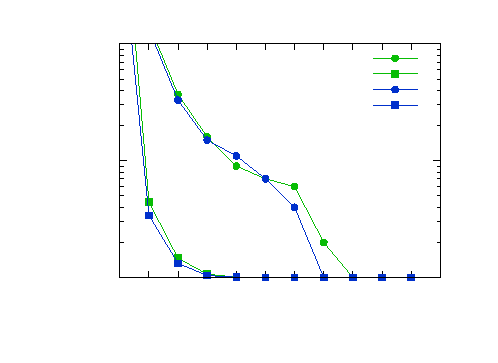
\includegraphics{../plots/authmodules-fga}}%
    \gplfronttext
  \end{picture}%
\endgroup

    \end{tabular}
    \caption[Results for number of crypto modules experiment]{The number of encryption modules (left column) and authentication modules (right column)
    is shown in relation to the maximum and average wait times of enqueued flits. Each row represents one protocol variant.}
    \label{fig:resultscryptomodules}
\end{figure}

\section{Experiments}
Record:
- acceptance rate (aka actual injection rate)
- information rate (source flits / total flits)
- residual error probability
- end-to-end latency
\subsection{Number of ARQs modified/dropped by routers}
\subsection{Routing strategies effects}
% Heatmap of router workload?

\iffalse
Experiment setup parameter tables:
- NC mode (UC, G2C3, G2C4)
- ...

ARQ Limit: 1, at most 2 because more ARQs allowed per transmission unit means larger retransmission buffers everywhere

\section{Statistics}
\begin{itemize}
    \item Injection/acceptance rate: [0, 1] (at processing element and at network interface)
    \item Queue lengths and buffer sizes
    \item Workload of crypto units
    \item Average/max flit waiting time at entry guard
    \item Average/max hop count
\end{itemize}

\section{Area Overhead}
\fi
